\subsection{Poisson}
Nochmal: die grundlegende Annahme von Seung-Hoon Na und Hwee Tou Ng lautet:\\
\fbox{ 
\begin{minipage}{12cm}
	``Our key assumption is that the frequency of anaphoric expressions is distributed over named entities in a document according to the probabilities of whether the document is elite for the named entities.''\cite{paper:Na}
\end{minipage}
}\\
\\
Um diese Annahme in ein mathematisches Modell zu übersetzen, muss man die Wahrscheinlichkeit abschätzen, dass ein Dokument ``elite'' ist. Wir suchen also eine Formel für
\[P\left( E\left( e \right)=1|d \right)=\ ?\]
Zunächst interessiert uns hierfür die Wahrscheinlichkeit, dass eine beliebige Entität tf-fach in einem Dokument vorkommt. Dafür wird ein 2-Poisson Mixture Modell herangezogen.
\[P\left( tf \right)=\pi_e\frac{e^{-\lambda_e}\lambda_{e}^{ tf }}{tf!}+\left( 1-\pi_e \right)\frac{e^{-\mu_e} \mu_e^{tf}}{tf!}\]
Der erste Term repräsentiert hierbei die Wahrscheinlichkeit des tf-fachen Auftretens der Entität in der Funktion als ``elite''-Eigennamen, der zweite Term steht für die Wahrscheinlichkeit des tf-fachen Auftretens der Entität als ``non-elite''-Eigennamen.
\[P\left( tf \right)=\underbrace{\pi_e\frac{e^{-\lambda_e}\lambda_{e}^{ tf }}{tf!}}_{Wahrscheinlichkeitsanteil - elite} +\underbrace{\left( 1-\pi_e \right)\frac{e^{-\mu_e} \mu_e^{tf}}{tf!}}_{Wahrscheinlichkeitsanteil - nonelite}\]
Dabei deutet $\pi_e$ auf den Erwartungswert hin, ob ein Dokument ``elite'' ist oder nicht.\\
$\pi_e$, $\lambda_e$ und $\mu_e$ werden festgelegt als:
\[\pi_e=\frac{df\left( e \right)}{df\left( e \right)+N}, \ \lambda_e=\frac{cf\left( e \right)}{df\left( e \right)}, \ \mu_e=\frac{cf(e)}{N}\]
Damit haben wir ein Modell, dass die Wahrscheinlichkeit der Häufigkeit von Entitäten in Dokumenten schätzt. Wichtig ist hierbei, dass sowohl das Auftreten von ``elite''-Entitäten in Dokumenten mit einer Poissonverteilung modelliert wird, als auch das ``zufällige'' Auftreten der ``nonelite''-Entitäten.\\
Eine einfache Poissonverteilung sieht in Formel und im Diagramm wie folgt aus:
\[P_\lambda(k)=\frac{\lambda^k}{k!}e^{-\lambda}\]
\begin{table}[h]
	\centering
	\begin{tabular}{c}
		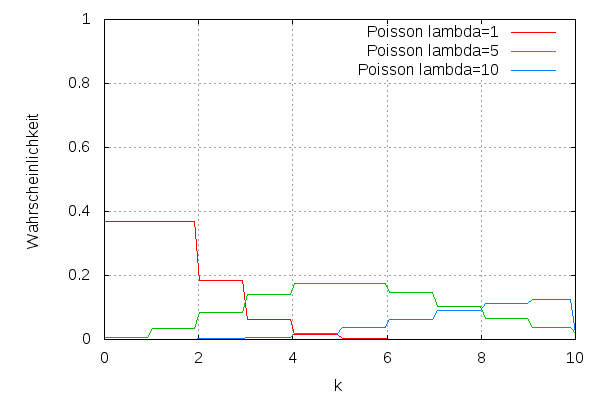
\includegraphics[scale=0.5]{pics/poisson_basic}
	\end{tabular}
	\caption{Einfache Poissonverteilung}
	\label{tab:poisson_basic}
\end{table}
